\documentclass[stu,12pt,floatsintext,a4paper]{apa7}
% English bachelor template (APA7, Uni Graz style)
% -------------------------------------------------
% Students: Use this file for an English bachelor thesis.
% Edit ONLY the metadata block below and the main content.
% Do NOT change package settings unless you know LaTeX.

\usepackage{booktabs}
\usepackage{multirow}
\usepackage[american]{babel}
%\usepackage[ngerman]{babel} % German only (see bachelor_ger.tex)
\usepackage{csquotes}
\usepackage[style=apa,sortcites=true,sorting=nyt,backend=biber]{biblatex}
% biblatex: loads the package that will handle the bibliographic info.
% - style=apa: sets the reference format to use apa (albeit the 6th edition)
\DeclareLanguageMapping{american}{american-apa}

% Optional: ensure English caption names/list titles are set explicitly.
\addto\extrasamerican{%%
    \renewcommand{\figurename}{Figure}%%
    \renewcommand{\tablename}{Table}%%
    \renewcommand{\listfigurename}{List of Figures}%%
    \renewcommand{\listtablename}{List of Tables}%%
}

% Bibliography file
\addbibresource{bibliography.bib}
\usepackage[T1]{fontenc}
\usepackage{mathptmx}

% Title page stuff _____________________
% =================== USER EDITABLE METADATA ===================
% Students: Edit ONLY the commands below. Do NOT change other
% parts of this file unless you know what you're doing.
% - Replace the values inside the braces for these commands.
% - Keep the command names intact so the template keeps working.
% ---------------------------------------------------------------
\newcommand{\thesisTitle}{"{A} Life in Word": Why It Makes Sense To Use LaTeX}
\newcommand{\thesisSemester}{Winter term 2018/19}
\newcommand{\thesisSupervisor}{Assoc. Prof. Dr. Harry Hirsch}
\newcommand{\thesisAuthor}{Susi Sorglos}
\newcommand{\department}{Biological Psychology}
\newcommand{\thesisDate}{2019-02-04}
\newcommand{\shortTitle}{Word is not good}
% ---------------------------------------------------------------
% End of USER EDITABLE METADATA
% ===============================================================

% Document language: fixed to English for this template.
\selectlanguage{american}

\title{Bachelor Thesis: \thesisTitle} % Full title for the title page
\shorttitle{\shortTitle} % Short title for headers
\author{\thesisAuthor}
\duedate{\thesisSemester}
% The student version doesn't use the \date command.
\affiliation{Institute of Psychology, University of Graz \\ \vspace{1cm} \includegraphics[width=3cm]{figures/uni-graz-logo.pdf}}
% No course field: simplified for students
\professor{\thesisSupervisor}

\begin{document}

% Custom Title Page (English version)
\begin{titlepage}
    \thispagestyle{empty}

    \noindent
    \begin{minipage}[c]{0.2\textwidth}
        \mbox{} % Empty box for spacing
    \end{minipage}%
    \begin{minipage}[c]{0.6\textwidth}
        \centering
        {\fontsize{32}{40}\selectfont \textbf{Bachelor Thesis}\\}
    \end{minipage}%
    \begin{minipage}[c]{0.2\textwidth}
        \raggedleft
        \includegraphics[width=0.8\linewidth]{figures/uni-graz-logo.pdf}
    \end{minipage}

    \vspace{1cm}

    \centering
    {\normalsize Within the course\\}
    \vspace{0.3cm}
    {\normalsize Seminar Research Methods in a Basic or Applied Subject: \department\\}
    \vspace{0.3cm}
    {\normalsize \thesisSemester\\}

    \vspace{1.5cm}

    {\Large \textbf{\thesisTitle}\\}

    \vspace{1.5cm}

    {\Large \thesisAuthor\\}

    \vspace{1.5cm}

    {\normalsize Submitted on \thesisDate \\}
    \vspace{0.3cm}
    {\normalsize Institute of Psychology \\}
    \vspace{0.3cm}
    {\normalsize University of Graz \\}
    \vspace{0.3cm}
    {\normalsize Supervisor: \thesisSupervisor \\}
\end{titlepage}
\newpage

% Acknowledgments
\section*{Acknowledgments}
I would like to thank my colleagues, mentors, and family for their support during the course of this study.
\newpage

% Abstract
\section*{Abstract}{This is the abstract for this paper, where the main points of the introduction, method, results, and discussion are briefly described. Probably in more than one sentence, though.}
\newpage

Begin your paper with the introduction. The active voice, rather than the passive voice (i.e., the zombie voice), should be used in your writing.

Since the Introduction is where references in papers first show up, let us incorporate some now. Referencing is done for us with the right command, like  \textcite{Sample2024}. But maybe you want to just include it all as a: \textbf{parenthetical}? \parencite{Fink2021, Contributor2023, Sample2024}.

\section{Method}

\subsection{Participants}

Talk about the people who participated in your study. How many students, sourced from where, reimbursed how, ethics assured by what?

\begin{table}[ht]
\centering
\caption{Demographics of Participants Included in the Study}
\begin{tabular}{lcccccc}
\toprule
\multirow{2}{*}{Participant ID} & \multirow{2}{*}{Age} & \multirow{2}{*}{Sex} & \multicolumn{2}{c}{ADS Score} \\
\cline{4-5}
 & & & Male & Female \\
\midrule
P001 & 29 & Male & 15 & - \\
P002 & 34 & Female & - & 12 \\
P003 & 41 & Male & 18 & - \\
P004 & 27 & Female & - & 14 \\
P005 & 38 & Male & 16 & - \\
P006 & 31 & Female & - & 13 \\
P007 & 45 & Male & 20 & - \\
P008 & 33 & Female & - & 17 \\
\bottomrule
\end{tabular}
\label{tab:demographics-eng}
\end{table}

\subsection{Materials}

Sometimes it can be helpful to include the stimuli used in the experiment. For example, here is an example table (Table \ref{tab:table_words-eng}) of words that were used in this hypothetical experiment. If you make use of the label command, \LaTeX{} will handle numbering things for you.

\begin{table}
    \caption{Sample words from this hypothetical experiment.}
    \centering
    \begin{tabular}{cc}
        \hline 
         First word & Second word \\
         \hline
         Yeet & Yoink \\
         Hot & Lit \\
         \hline
    \end{tabular}
    \label{tab:table_words-eng}
\end{table}

\section{Results}

Some instructors will want things broken down with the subheadings (e.g., `Descriptive Statistics') I have included, some will be unhappy if you \textit{do} include these. Always check with the assignment/rubric for what is wanted.

\subsection{Descriptive Statistics}

In this portion, you describe the data obtained. This includes things like the counts, means, and standard deviations. This may be omitted or rolled into the rest of the statistical discussion, so as always, check with what is being asked of you.

\begin{figure}
    \centering
    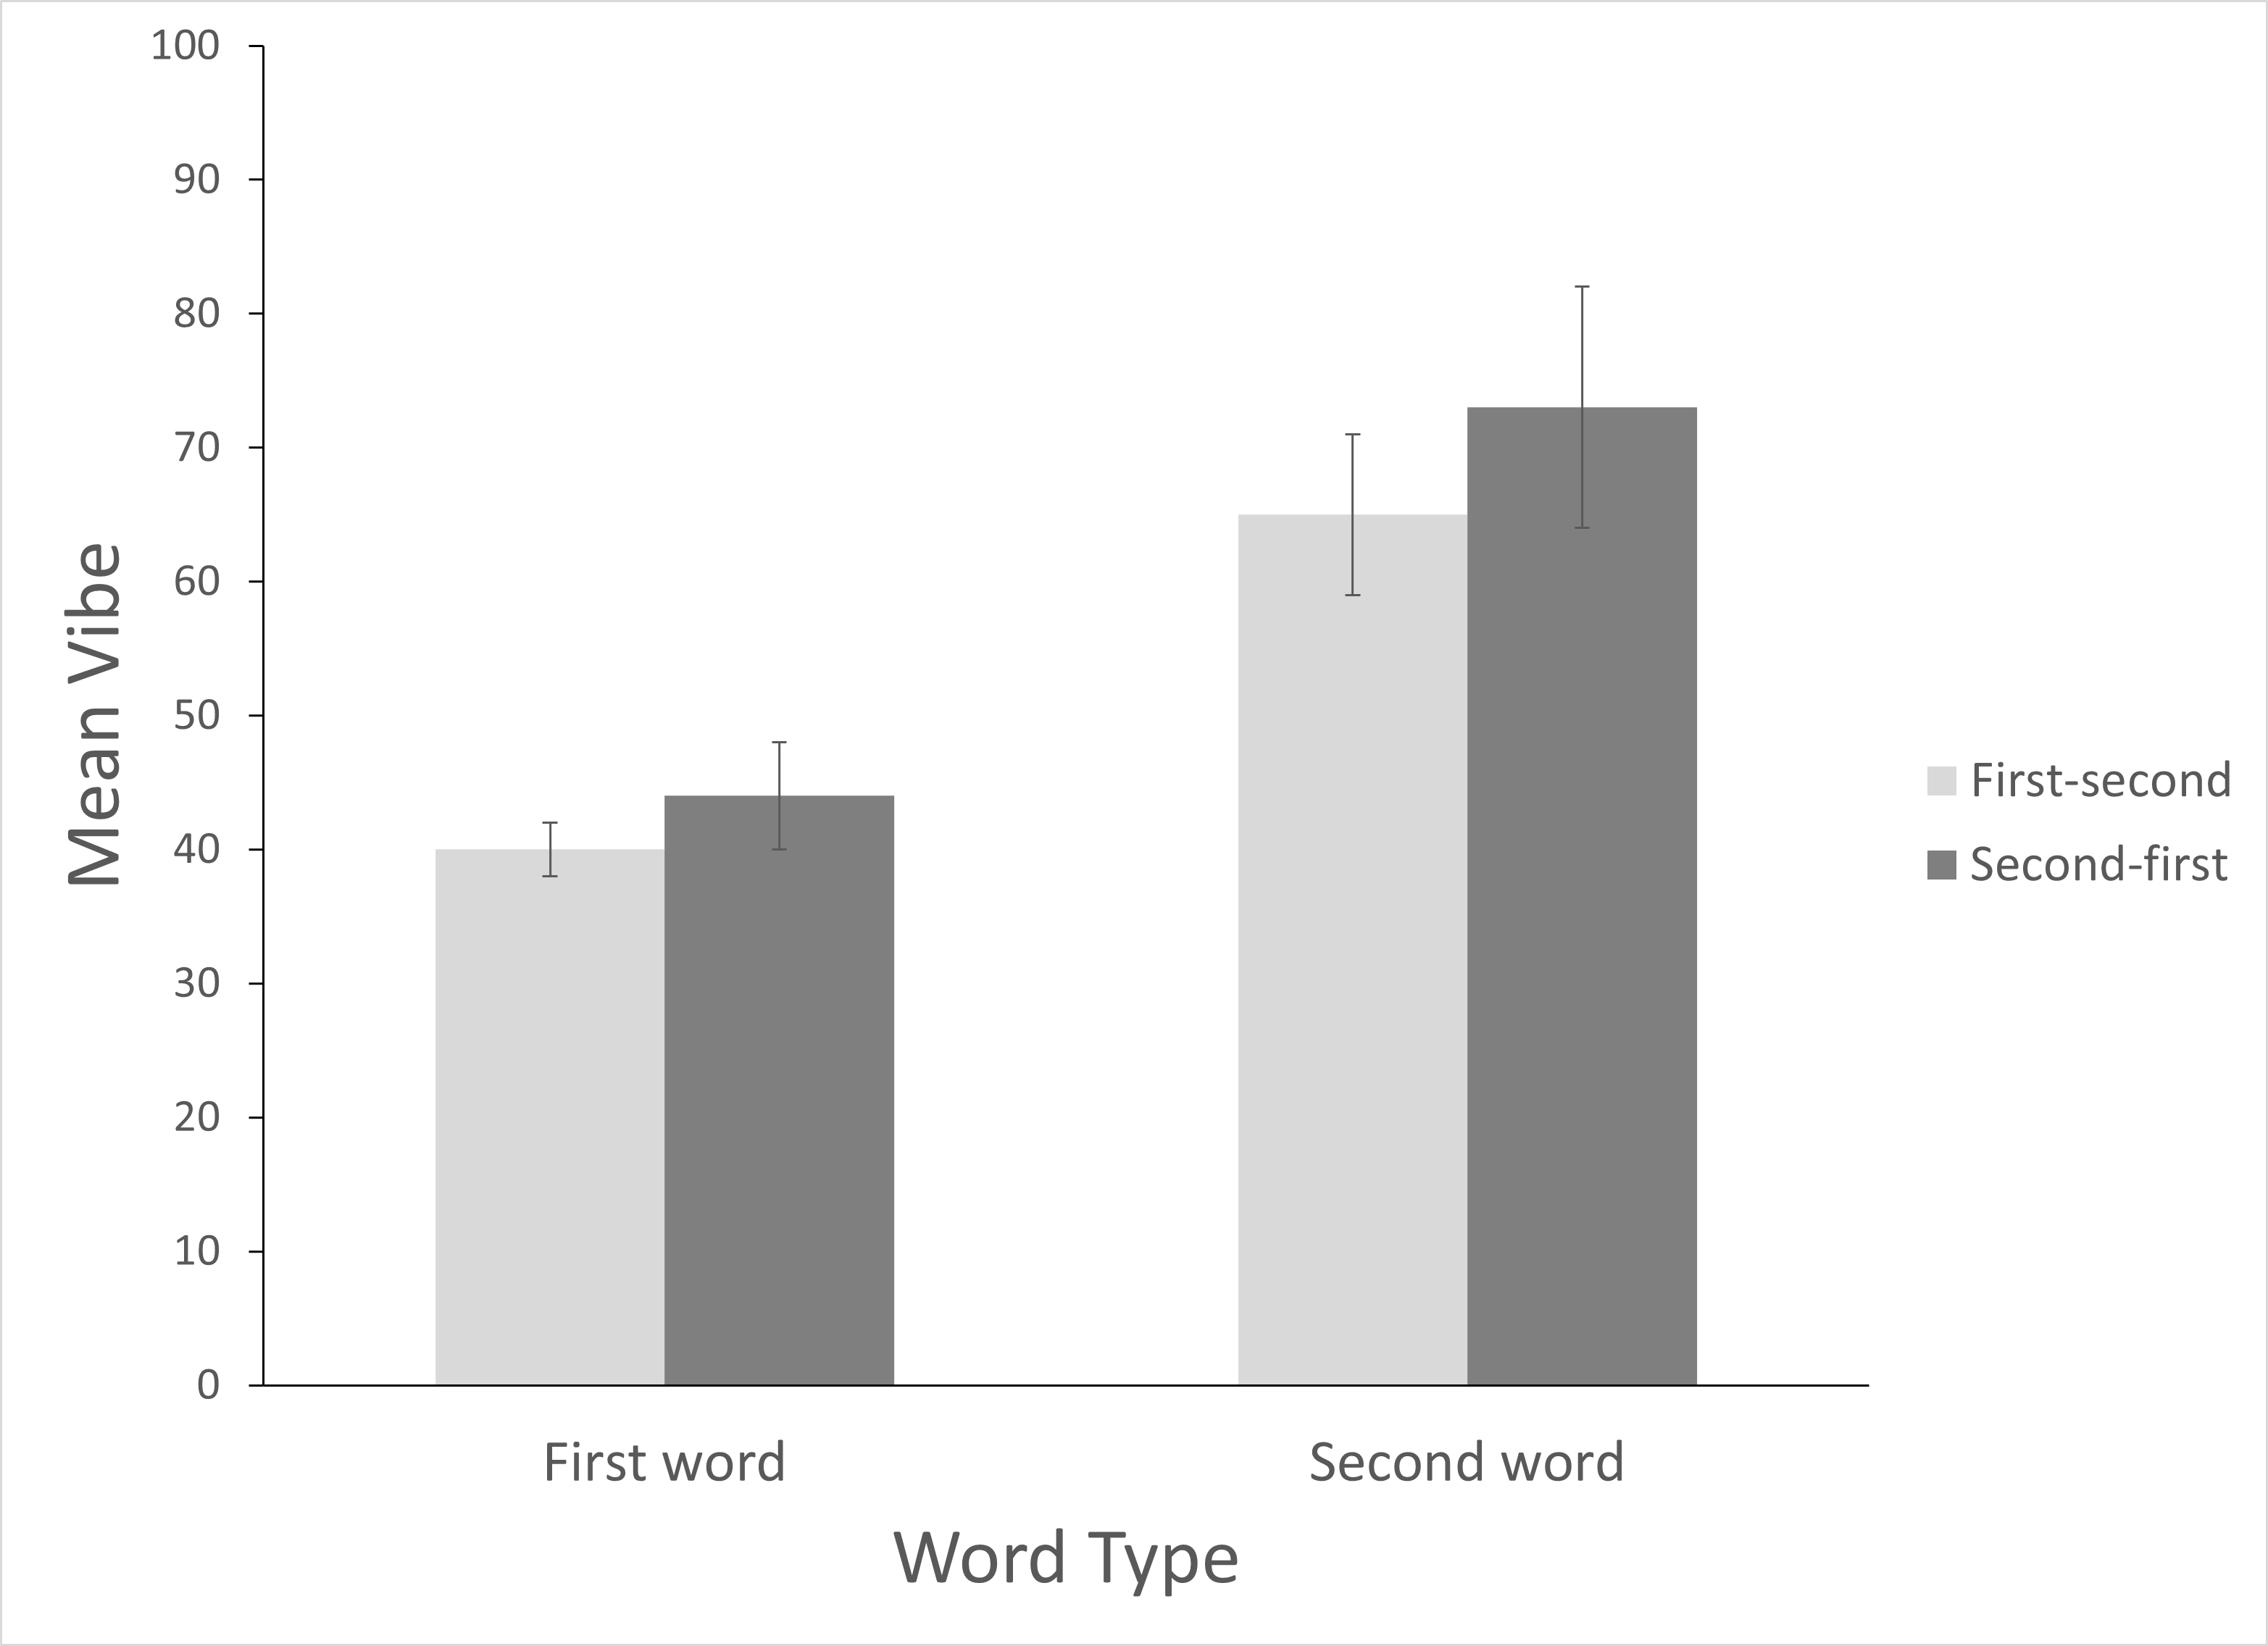
\includegraphics[width=0.75\linewidth]{figures/sampleFig.png}
    \caption{The mean vibes for each word type and counterbalanced condition order. Error bars represent one standard error of the mean.}
    \label{fig:OverallEffect-eng}
\end{figure}

Figure~\ref{fig:OverallEffect-eng} shows the means and standard errors for the four experimental groups. As shown, the mean vibes for the second word ($M = $ 69, $SE = $ 7.5) were greater than the first word ($M = $ 42, $SE = $ 3), but roughly equivalent between presentation order conditions.

\subsection{Inferential Statistics}

This is where you start to do the actual statistical analysis. We generally tell students not to \textit{interpret} what the results mean until the discussion, but pay attention when reading journal articles - realistically a bit of interpretation does tend to happen at this point in published works.

% Example macros for reporting statistics
\newcommand{\ttestSig}[2]{$t$(#1) = #2, $p < .05$}
\newcommand{\ttestInsig}[2]{$t$(#1) = #2, $p > .05$}
\newcommand{\anovaSig}[3]{$F$(#1,#2) = #3, $p < .05$}
\newcommand{\anovaInsig}[3]{$F$(#1,#2) = #3, $p > .05$}

Using the hypothetical experiment we have set up, let's say there was a significant interaction found between the word conditions (first versus second) and exposure order (first-second versus second-first), \anovaSig{11}{111}{4.20}. Pairwise comparisons indicate that this was driven by the words themselves, as there was a significant difference between the words, \ttestSig{111}{3.21}, but not for the exposure order, \ttestInsig{111}{.42}.

\section{Discussion}

As mentioned at the close of the Introduction, the Discussion starts out specific before building out to the broader picture. This will typically mean that the discussion starts with a reiteration of the Results, with more emphasis on interpretation.

With that done, you can work to tie your findings into the existing literature. Perhaps this result supports the work of \textcite{Contributor2023} but contradicts others \parencite[e.g.,][]{Sample2024}.

Finally, close things out by reiterating the brief version of your findings, what it means for the theory you were testing, and what it could mean for future research.

\printbibliography

\end{document}
